This chapter outlines and motivates the main objectives of the project. First, the importance of the analysis of coral skeletons is discussed. Next, the motivations for an automated analysis process are outlined and the choice of a deep learning based solution is justified. The challenges involved in completing the project are highlighted, and related works in the analysis of coral skeletons are then briefly discussed. Finally, the main objectives of the project are summarised and listed.

\section{Introduction}

Coral polyps are tiny soft-bodied organisms. Through a process known as calcification, they use calcium and carbonate ions from the surrounding seawater to build themselves hard calcium carbonate skeletons. These polyps reproduce asexually and can form colonies of up to thousands of individual polyps all contributing to the same connected skeleton.

Using X-radiographs in 1972, Knutson et al. were able to confirm the presence of annual density bands in these calcium carbonate skeletons~\cite{knutson}. An annual density band consists of two portions: a high-density portion produced during the late summer and a low density portion formed during periods of seasonally lower water temperatures~\cite{highlow}. These bandings are parallel to the growth surface and orthogonal to the direction of growth; examples are shown in Figure \ref{fig:densityexample}. With knowledge of a coral sample's date of collection, these annual band pairs can be counted back through time to provide not only an age of the sample, but also a chronology of the coral's growth. More specifically, the annual banding can be used to measure three aspects of coral growth~\cite{lough2011new}:

\begin{enumerate}
    \item The linear extension rate (mm y$^{-1}$): the distance that the coral grows per year.
    \item The density (g cm$^{-3}$): the density of the skeletal matter being produced.
    \item The calcification rate (g cm$^{-2}$ y$^{-1}$): the mass of skeletal matter being produced per year, calculated by multiplying the linear extension rate with the density.
\end{enumerate}

Analysis of these aspects of growth can be used to determine changes in a coral sample's environmental conditions as it was growing. Lough and Cooper highlight one significant potential use of the banding information contained within coral skeletons: ``skeletal material contained deep within massive corals can be extracted to allow comparisons of present day growth rates with those pre-dating the industrial revolution and hence examine the consequences of climate and environmental changes on coral reefs''~\cite{lough2011new}.

This project aims to automate the estimation of the linear extension rate which can then used to estimate the calcification rate. Deep learning will be used to extract the boundaries of each annual density band and the distance between these boundaries will then be estimated using various methods based off of the Hausdorff distance.

\begin{figure}[t]
    \centering
    \begin{subfigure}[t]{0.49\textwidth}
        \centering
        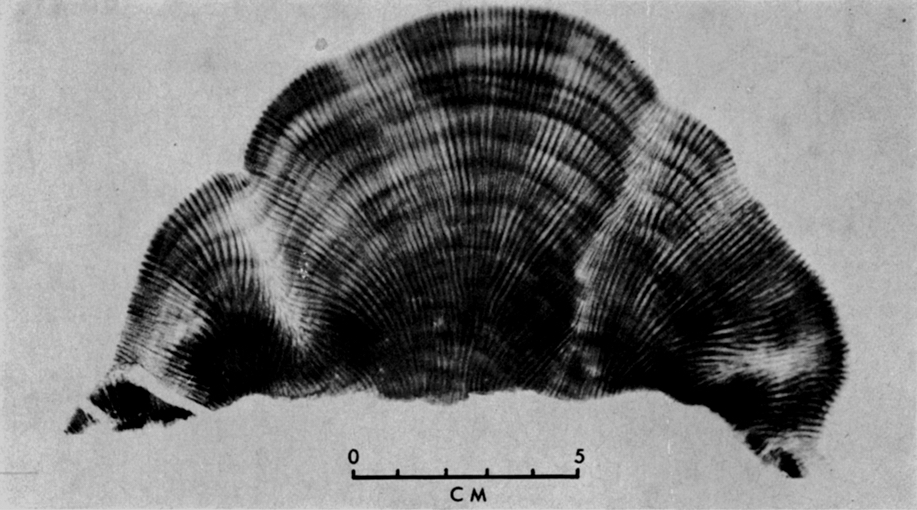
\includegraphics[width=1\textwidth, valign=c]{images/knutson.jpg}
    \end{subfigure}
    ~
    \begin{subfigure}[t]{0.49\textwidth}
        \centering
        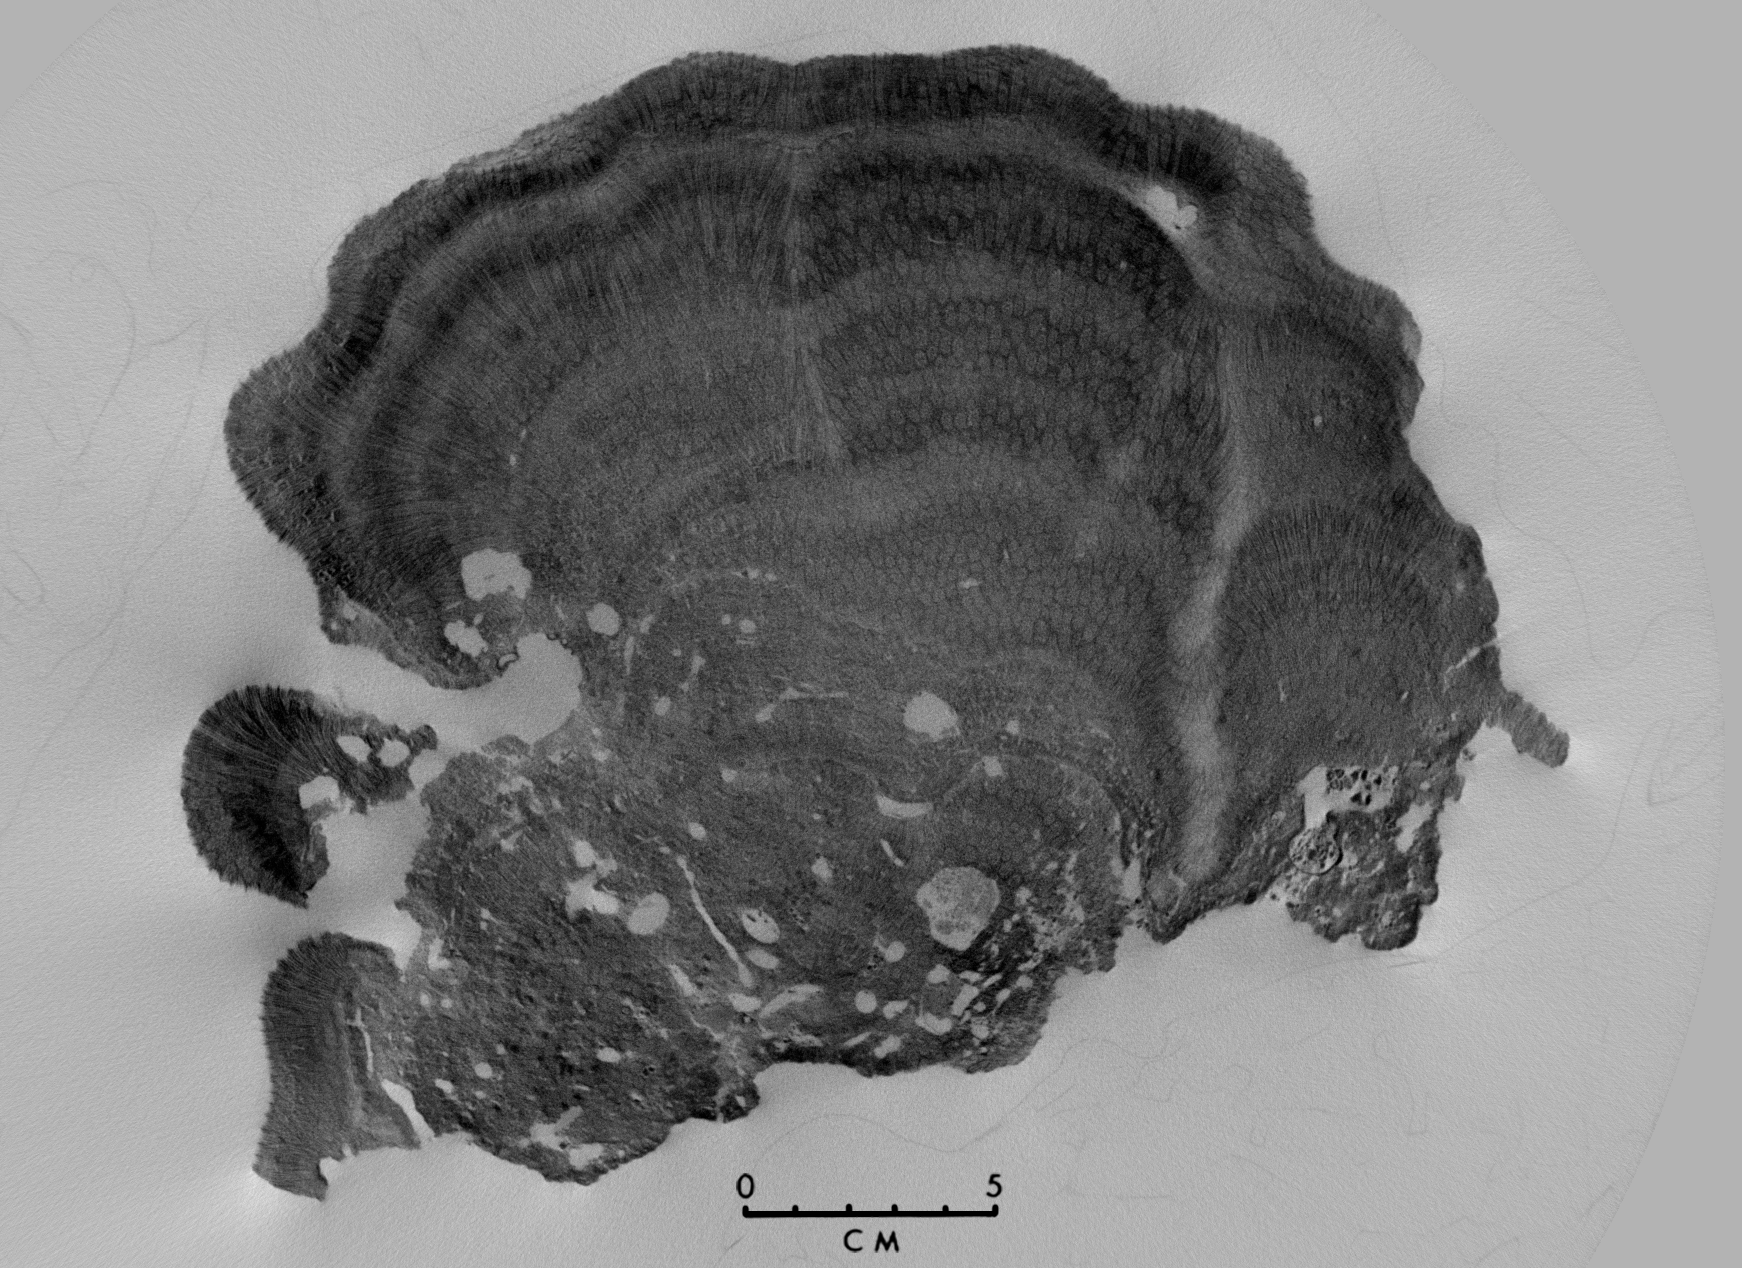
\includegraphics[width=1\textwidth, valign=c]{images/our-coral.png}
    \end{subfigure}
    \caption{Examples of the annual density bands present in the skeletons of a genus of coral called Porites. \textbf{(left)} An X-radiograph of a Porites lobatu coral sample presented by Buddemeier, Maragos, and Knutson in 1974: ``[this is a] positive print of the X-ray negative; dark images correspond to high skeletal density, light images to low density''~\cite{coralimage}. \textbf{(right)} An image taken from one of the CT scans of a Porites sample from the dataset used in this project. The image channel has been inverted resulting in dark pixels corresponding to high density, and light pixels corresponding to low density.}
    \label{fig:densityexample}
\end{figure}

\section{Motivations}

% This section discusses the need for an automated solution and attempts to justify the choice of a deep learning based solution.

\subsection{An Automated Solution}

Although many methods for manually estimating the linear extension and calcification rates exist, an automated solution could be beneficial for multiple reasons.

Firstly, opinions on the positions of a particular boundary between high and low density bands can differ from person to person. It is important to note that an idealised annual density cycle is actually in the form of a sinusoidal wave with the density gradually changing from high to low and back over the course of a year~\cite[p. 39]{coralsine}. Thus, an exact boundary between a high and low band does not actually exist. However, an effort can be made to consistently choose boundaries at the same point in the sinusoid each year. Naturally, people can disagree with each other when determining the positions of the boundaries; a researcher labelling the same slice for a second time might even disagree with their previous choices of boundary positions. This is not the case, however, for an artificial neural network. Once trained, a neural network is deterministic; given a particular input, it will always produce the same output.

Another benefit of the proposed automated solution is speed. An example of a manual solution is to manually label the density boundaries, use a tool to measure distances between multiple points along these boundaries, and average the distances measured to produce a single average linear extension rate. This process can be time consuming. The proposed solution could potentially estimate the calcification rate of a given slice in a matter of seconds. This could allow researchers to not only analyse the density banding quicker, but may also ultimately enable them to process more data overall.

Finally, an automated solution could potentially be more accurate than a manual solution. For example, an automated solution could measure hundreds of distances between two boundaries which could be used to produce a more accurate estimate than a manual solution in which only tens of distances were averaged.

\subsection{Deep Learning}
\label{sec:contextdl}

Feed-forward artificial neural networks have existed in some form since 1965~\cite{deepoverview, 1966cybernetic}, but the term ``deep learning'' was only coined in 2006~\cite{deepoverview, hintondeep, hintonfast}. In the years since, the field of deep learning has seen a significant rise in both its popularity and practicality for a multitude of reasons and is now the state-of-the-art in many areas. This section outlines the justifications of the choice of a deep learning based solution. Deep learning is discussed in more technical detail in Section \ref{sec:deeplearning}.

\subsubsection{The Dataset}

This project will make use of a dataset of more than 160 three dimensional computed tomography (CT) scans of unique coral skeletons from the Natural History Museum's collection. These three dimensional scans are stored as stacks of two dimensional \texttt{.tif} images. With each scan being represented by ${\sim}2000$ images, the whole dataset consists of hundreds of thousands of images. The raw dataset provided is unlabelled, so in order to train a supervised machine learning model\textemdash such as an artificial neural network\textemdash to extract the boundaries, some of the data must be manually labelled.

Although the labelling process is time consuming and will not be possible for the entire dataset, the hope is that researchers at the University of Bristol and the Natural History Museum can continue to label and re-train the proposed system even after this project is over. The abundance of data available makes a deep learning based solution a reasonable choice.

\subsubsection{Semantic Segmentation}
\label{sec:semseg}

The task of extracting the boundaries between density bands can be presented as a semantic segmentation task. The volumetric CT data can be broken down into two dimensional images and from there, each pixel will be given a label from one of two classes: part of a boundary or not part of a boundary (see Figure \ref{fig:example-label}).

\begin{figure}[t]
    \centering
    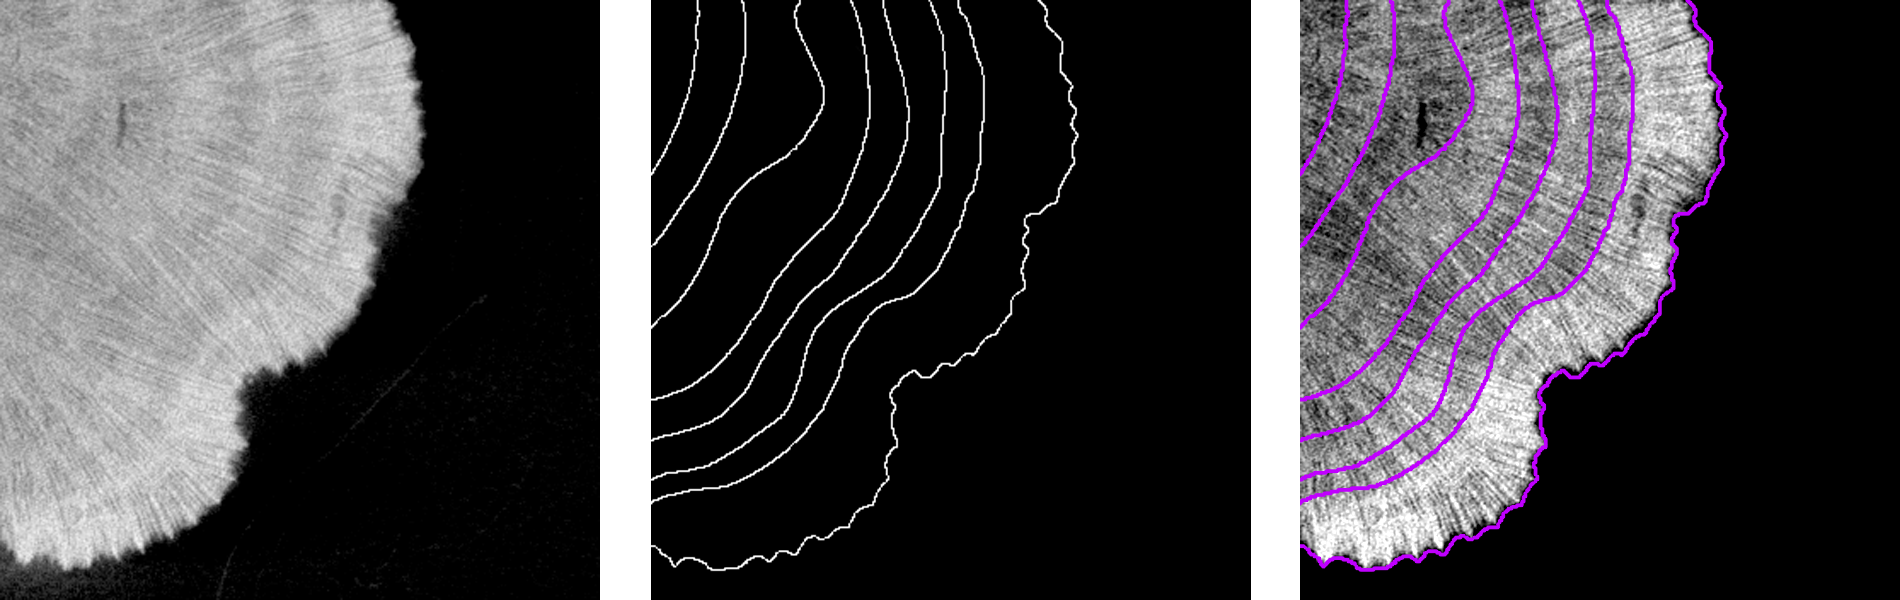
\includegraphics[width=1\textwidth]{images/label-example.png}
    \caption{An example of a manually labelled 2D slice. This represents the ideal semantic segmentation of a slice. \textbf{(left)} An unaltered section of a 2D slice taken from a 3D scan of a coral sample. \textbf{(centre)} The manual labelling of the section. The white pixels correspond to the ``part of a boundary'' class, and the black pixels correspond to the ``not part of a bounary'' class. \textbf{(right)} The manual labelling overlaid with the corresponding section of the slice. The contrast and brightness of the slice has been altered to better show the annual banding, and the colour of the labelling has been changed for illustration purposes.}
    \label{fig:example-label}
\end{figure}

Several forms of deep convolutional neural networks (CNNs) currently achieve the state-of-the-art in semantic segmentation\footnote{\url{https://paperswithcode.com/task/semantic-segmentation/latest}}~\cite{chen2018encoder, semanticseg-SOTA}. For this project, pre-existing CNN architectures used for semantic segmentation that perform well on existing datasets are a reasonable starting point. Several CNN architectures will be repurposed and/or modified to process the skeletal density data.

The main architecture experimented with will be the U-Net architecture~\cite{ronneberger2015u}. U-Net was initially used to perform semantic segmentation on biomedical images such as images of cells on glass recorded with differential interference contrast mi-croscopy. The U-Net architecture has not yet been applied to coral density data and experimentation with the U-Net architecture and the dataset used in this project could yield interesting results. To the best of the author's knowledge, none of the architectures experimented with throughout this project have ever been applied to coral skeleton density data of any kind. This project aims to not only determine how well multiple architectures perform in segmenting the skeletal density data but also to determine if CNNs are currently a viable solution to this task.

\section{Challenges}

% There are multiple challenges involved in the implementation of an automated solution. This section outlines and briefly discusses the most significant of these challenges.

\subsection{Labelling}

As previously discussed, the process of manually labelling the boundaries present in the data is time consuming. Labelling enough data for a CNN to perform well would require tens of hours of work. This process takes particularly long as appropriate slices must be extracted from the 3D CT data using a 3D visualisation program such as Avizo\footnote{\url{https://tiny.cc/avizo}} before they can be labelled. Not only is this process time consuming, it is also challenging. This is especially the case for a person that has not dealt with coral skeleton density data before. Before samples can be manually labelled, an acceptable standard of labelling must be approved by an expert.

\subsection{Class imbalance}

Another challenge involved with this project is dealing with the inherent class imbalance of the boundary labels. In a typical classification problem, class balance occurs when one class contains significantly fewer samples than the other classes. Since semantic segmentation can be seen as per-pixel classification, class imbalance can be an issue in this task as well. Looking at Figure \ref{fig:example-label}, it can be seen that the ratio of white to black pixels in the label is significantly low. There is a severe class imbalance between the ``part of a boundary'' and ``not part of a boundary'' classes. When a class imbalance exists within training data, supervised learning models will typically over-classify the ``majority'' groups due to their increased prior probabilities. As a result, the instances belonging to ``minority'' groups are misclassified more often than those belonging to the majority groups~\cite{classimbalance}.

This class imbalance gives rise to another challenge when assessing the performance of a model in its segmentation of the density data. Since the boundary labels are only one pixel wide, a model predicting boundary positions just one pixel to the left or right could achieve an accuracy of 0\%. To solve this problem, a custom accuracy metric must be conceived in order to reward a model even in predicting a boundary a few pixels away from the manually labelled position.

\subsection{Loading Three Dimensional Data}

When implementing an architecture capable of segmenting data in three dimensions, existing deep learning libraries\textemdash such as the Keras\footnote{\url{https://keras.io/}} library used throughout this project\textemdash make the implementation of a 3D architecture relatively straightforward. However, as of the time of writing, a 3D ``data loader'' capable of loading 3D data from a directory and performing online data augmentation does not yet exist for the Keras library and would have to be designed and implemented.

\section{Related Work}

Although there exists many examples of coral species classification using deep learning, no machine learning techniques of any kind have been applied to CT scans of coral skeletons. The implementation of an automated system to extract the density banding or calculate the linear extension and calcification rates has not yet been attempted or at least published.

Steffens et al.~\cite{steff} make use of the DeeplabV3~\cite{deeplab} CNN to segment coral reef images into different types of substrates. However, the ImageCLEFcoral\footnote{\url{https://www.imageclef.org/2019/coral}} dataset that they use to test their implementation consists of images taken of the surfaces of coral reefs. Alonso et al.~\cite{alonso} segment coral reef images of a similar kind from the Eilat Fluorescence Corals dataset~\cite{eilat} using the SegNet CNN architecture~\cite{segnet}. Again, this work attempts to segment images taken of the surfaces of coral reefs rather than any kind of data representing the internals of a coral skeleton.

Three dimensional implementations of the U-Net architecture do exist. For example, {\c{C}}i{\c{c}}ek et al.~\cite{cicek} modify the U-Net architecture to process 3D data by replacing all 2D operations with their 3D counterparts. They assess the performance of their model on a dataset of Xenopus kidney embryos and propose both semi-automated and fully-automated use cases of the model. It is worth noting that the segmentation task that they are attempting does not give rise to a class imbalance. The nature of the segmentation this project will attempt is dissimilar due to the sparsity of the density boundaries.

% {\bf A compulsory chapter,     of roughly $5$ pages}
% \vspace{1cm} 

% \noindent
% This chapter should describe the project context, and motivate each of
% the proposed aims and objectives.  Ideally, it is written at a fairly 
% high-level, and easily understood by a reader who is technically 
% competent but not an expert in the topic itself.

% In short, the goal is to answer three questions for the reader.  First, 
% what is the project topic, or problem being investigated?  Second, why 
% is the topic important, or rather why should the reader care about it?  
% For example, why there is a need for this project (e.g., lack of similar 
% software or deficiency in existing software), who will benefit from the 
% project and in what way (e.g., end-users, or software developers) what 
% work does the project build on and why is the selected approach either
% important and/or interesting (e.g., fills a gap in literature, applies
% results from another field to a new problem).  Finally, what are the 
% central challenges involved and why are they significant? 
 
% The chapter should conclude with a concise bullet point list that 
% summarises the aims and objectives.  For example:

% \begin{quote}
% \noindent
% The high-level objective of this project is to reduce the performance 
% gap between hardware and software implementations of modular arithmetic.  
% More specifically, the concrete aims are:

% \begin{enumerate}
% \item Research and survey literature on public-key cryptography and
%       identify the state of the art in exponentiation algorithms.
% \item Improve the state of the art algorithm so that it can be used
%       in an effective and flexible way on constrained devices.
% \item Implement a framework for describing exponentiation algorithms
%       and populate it with suitable examples from the literature on 
%       an ARM7 platform.
% \item Use the framework to perform a study of algorithm performance
%       in terms of time and space, and show the proposed improvements
%       are worthwhile.
% \end{enumerate}
% \end{quote}

\section{Summary of Objectives}

In summary, the main objective of this project is to automate the estimation of the calcification rate\textemdash the amount of skeletal matter produced annually by corals. This objective is broken down into multiple tasks:

\begin{enumerate}
    \item Curate a dataset of image-label pairs from the raw unlabelled dataset provided.
    \item Train existing two dimensional convolutional neural network architectures to extract the annual density boundaries present in the data.
    \item Modify the architectures to process three dimensional data.
    \item Conceive and implement an accuracy metric to assess the performance of different networks on the data.
    \item Optimise hyper parameters of the chosen network architecture to maximise accuracy.
    \item Make use of these extracted boundaries to automate the calculation of the annual skeletal matter produced.
    \item Package the implementation in a form usable by researchers at the Natural History Museum and the School of Earth Sciences at the University of Bristol.
\end{enumerate}
